\documentclass[11pt,a4paper]{article}
\usepackage[T1]{fontenc}
\usepackage[margin=1in]{geometry}
\usepackage{amsmath,amssymb,amsthm,mathtools}
\usepackage{booktabs}
\usepackage{graphicx}
\usepackage{xcolor}
\usepackage[colorlinks=true,linkcolor=blue!60!black,citecolor=blue!60!black,urlcolor=blue!60!black]{hyperref}
\usepackage{microtype}
\usepackage{enumitem}
\usepackage[most]{tcolorbox}
\usepackage{listings}
\lstset{language=Python,basicstyle=\ttfamily\scriptsize,breaklines=true,columns=fullflexible,keepspaces=true,frame=single,framerule=0.3pt,xleftmargin=4pt}
\newcommand{\lean}[1]{\texttt{\small #1}}
\newcommand{\PENDING}[1]{\textcolor{red!70!black}{[pending: #1]}}
\newtcolorbox{keybox}[1][]{colback=blue!3,colframe=blue!45!black,boxrule=0.5pt,left=4pt,right=4pt,top=3pt,bottom=3pt,#1}
\newtcolorbox{failbox}[1][]{colback=red!3,colframe=red!45!black,boxrule=0.5pt,left=4pt,right=4pt,top=3pt,bottom=3pt,#1}

\title{\textbf{The friction on a quantized vortex in a truncated Gross--Pitaevskii field follows the temperature, not the normal density}\\
\large A pre-registered test of $\alpha\propto\rho_n$ against the cutoff, and the correction of a published reading}
\author{Xavier Callens\\ \small SocrateAI-Scientific-QuantumFluids\\
\small \url{https://github.com/xaviercallens/SocrateAI-Scientific-QuantumFluids}}
\date{October 2026}

\begin{document}
\maketitle

\begin{abstract}\noindent
The mutual friction $\alpha$ that drags a quantized vortex through the thermal component of a two-dimensional Bose
gas is commonly taken to scale with the normal fraction $\rho_n/\rho$. In an earlier paper~\cite{Callens2026a} we measured
$\alpha=0.0062$, $0.014$, $0.02$ at three temperatures of the projected Gross--Pitaevskii equation at one cutoff and
found $\alpha\simeq0.24\,\rho_n/\rho$; we read the coefficient as a mode-averaged transport cross-section of the
vortex, $1.4$ healing lengths, and registered the question of whether it depends on the cutoff, with the Born
phonon-scattering law as the rival ($\propto k_c$). We now measure $\alpha$ at two further cutoffs, $k_c\xi=2\pi/3$ and $2\pi$,
with the same energy-conserving instrument, with its $T=0$ known answer reproduced at each cutoff to $0.3\,\%$. The registered
prediction of a cutoff-independent coefficient fails, and so does its rival: the coefficient $c=\alpha/(\rho_n/\rho)$ is
$0.31\pm0.03$, $0.232\pm0.014$ and $0.102\pm0.011$ at $k_c\xi=2.1$, $3.1$, $6.3$, falling by a factor $3.1$ while $\rho_n/(\rho T)$
rises by a factor of three to four. What does not move is $\alpha$ itself: $\alpha/T=0.054\pm0.003$ in six arms ($\chi^2=1.3$ for $5$ degrees of freedom)
over three cutoffs and $T=0.10$--$0.22$ ($0.060\pm0.002$ with the regression estimator: the primary energy estimator is biased low by diffusion, a flaw of the registered synthetic gate that a second implementation exposed). The proportionality to $\rho_n$ reported before was a degeneracy of a single cutoff, where
$\rho_n\propto T$; the mode-averaged cross-section is not a property of the vortex ($1.9$, $1.4$, $0.59$ healing lengths) and the
``geometric core size'' reading is withdrawn. The temperature law was found after the data were read; it was registered as a hypothesis,
with its prediction for the next arm fixed in advance: $\alpha=0.0094\pm0.0010$ at $k_c=2\pi$, $T=0.173$, against $0.0077$ if the friction followed $\rho_n$. The arm gives $0.0096\pm0.0018$, inside the window registered for the temperature law --- a confirmation by the rule, although the error is almost twice the one assumed when the window was written, so the arm alone separates the two readings by one standard deviation; the discrimination rests on the comparison across cutoffs.
\end{abstract}

\section{Introduction}

The mutual friction on a vortex line in a superfluid is parametrised, in the Hall--Vinen form, by $\alpha$ (along the
relative velocity) and $\alpha'$ (across it). The standard microscopic picture, from phonon and roton scattering, makes the force proportional
to the density of excitations and hence $\alpha\propto\rho_n$~\cite{Iordanskii1964,Sonin1997}; measurements of the thermal friction on vortices in atomic condensates give values of order $10^{-2}$~\cite{Moon2015,Kwon2021}, and the only first-principles values for a
truncated Gross--Pitaevskii field come from vortex-pair dynamics in the Galerkin-truncated equation~\cite{Shukla2014}.

In the preceding paper~\cite{Callens2026a} we measured $\alpha(T)$ in the \emph{projected} Gross--Pitaevskii equation (PGPE), microcanonical,
with no damping term and no noise, with estimators that are identities of the dissipative point-vortex model. The result was
$\alpha=0.0062(4)$, $0.014(2)$, $0.02(1)$ at $T/T_{\rm BKT}=0.14$, $0.27$, $0.43$, and the ratio $\alpha/(\rho_n/\rho)=0.23$, $0.26$, $0.22$. That ratio is
the observation this paper tests. We had added an interpretation: for any isotropic bath the drag and the Landau normal density are sums over the same modes with the
same weight (Appendix~\ref{app:lean}), so $\alpha/(\rho_n/\rho)$ is the $w$-weighted mean of $c_g\sigma_{\rm tr}$ over the modes, which we evaluated at $1.4$
healing lengths, ``the geometric size of the core'', and we registered the cutoff dependence as the open question: if the coefficient is a property of the vortex
it should not depend on the cutoff that defines the bath; the Born law $\sigma_\parallel=\kappa^2k/8c^2$~\cite{Sonin1997}, extrapolated to the cutoff, predicts $c\propto k_c$.

\begin{keybox}
\textbf{Registered before any run} (\texttt{PGPE\_FRICTION\_LAW\_PREREG.md}, and the kinetic note of the same day): \textbf{FL1}, $\alpha\propto\rho_n$ at each cutoff;
\textbf{FL2}, the coefficient $c=\alpha/(\rho_n/\rho)$ differs between three cutoffs by less than $20\,\%$ (the rival: a shift above $40\,\%$ growing with $k_c$);
\textbf{FL3}, a spread of $10$--$30\,\%$, ordered $c(2\pi/3)\le c(\pi)\le c(2\pi)$, and the Born scaling $0.67:1:2$ as the sharp alternative.
\end{keybox}

\section{Instrument and data}\label{sec:method}

The instrument is that of the preceding paper: PGPE on a periodic box $L=64$ (units $\hbar=m=g=1$, mean density $1$), projector $|k|\le k_c$, symplectic split-step evolution with energy drift
below $10^{-4}$; antiparallel vortex pairs imprinted with the corrected phase-and-Bernoulli-amplitude profile in thermal base states; sub-grid vortex
tracking; $\alpha$ from the energy estimator $\alpha=-\Delta H/(2\int\!\sum|v_s|^2dt)$ and from a two-coefficient regression of the velocities; block jackknife errors;
runs end by annihilation or track loss and a validity cut $d\ge4$ is applied. The cutoffs are $k_c=\pi$ (the published arm, grid $N=128$), $k_c=2\pi/3$ (the same grid, projector at a third of the grid wavenumber) and $k_c=2\pi$ (grid $N=256$, $dx=\xi/4$).

\paragraph{Base states.} Each base is the equilibrated vortex-free $e=0.60$ state re-projected (and Fourier-resampled) under the new cutoff, heated to a target energy by the phonon construction, evolved
$1000$ time units, and measured over $500$ (temperature from the equipartition fit, $n_s/n=1-J_T/J_L$, raw vortex count); a base is admitted only if the vortex count is below $0.5$
(Table~\ref{tab:bases}). The fine-grid base at $T=0.217$ ($1.32$ vortices) failed admission; the second fine temperature is therefore $T=0.173$, not the registered $0.22$, and it
is the arm that was still running when the temperature law was formulated.

\begin{table}[h]\centering\small
\begin{tabular}{llrrrrl}\toprule
cutoff & grid & $e$ & $T$ & $n_s/n$ & $\rho_n/\rho$ & raw $n_v$ (admitted)\\\midrule
$2\pi/3$ & $N=128$ & 0.545 & 0.100 & 0.9846 & 0.0154 & 0.00\\
$2\pi/3$ & $N=128$ & 0.60 & 0.216 & 0.9603 & 0.0397 & 0.00\\
$\pi$ (published) & $N=128$ & 0.60 & 0.115 & 0.973 & 0.027 & 0.00\\
$\pi$ (published) & $N=128$ & 0.70 & 0.220 & 0.947 & 0.053 & 0.00\\
$2\pi$ & $N=256$ & 0.95 & 0.127 & 0.9291 & 0.0709 & 0.04\\
$2\pi$ & $N=256$ & 1.10 & 0.173 & 0.9198 & 0.0802 & 0.08\\
$2\pi$ & $N=256$ & 1.25 & 0.217 & 0.9029 & 0.0971 & 1.32 (\emph{not admitted})\\\bottomrule
\end{tabular}
\caption{Base states of the campaign. At comparable $T$ the normal fraction grows steeply with the cutoff ($\rho_n/\rho=0.015$, $0.027$, $0.071$ at $T=0.100$, $0.115$, $0.127$): the Landau sum runs over more modes.}\label{tab:bases}
\end{table}

\paragraph{Known answers.} At $T=0$ (uniform condensate, antiparallel $d_0=10$, $400$ time units) the pair moves at $0.1065$, $0.1068$, $0.1065$ ($k_c=\pi$, $2\pi/3$, $2\pi$) and the separation of the four-vortex
configuration oscillates between $9.7$ and $10.6$ with the same phase at all three cutoffs (Fig.~\ref{fig:t0}); $|\hat\alpha|\le5\times10^{-4}$ and $1-\hat\alpha'=0.9986$, $0.9995$, $0.9991$. The residual diffusion
floor is $2.9\times10^{-5}$ at $2\pi/3$ against a registered clause of $2\times10^{-5}$: marginal, reported, and a factor $10^{2}$ below the thermal values used below.

\begin{figure}[h]\centering
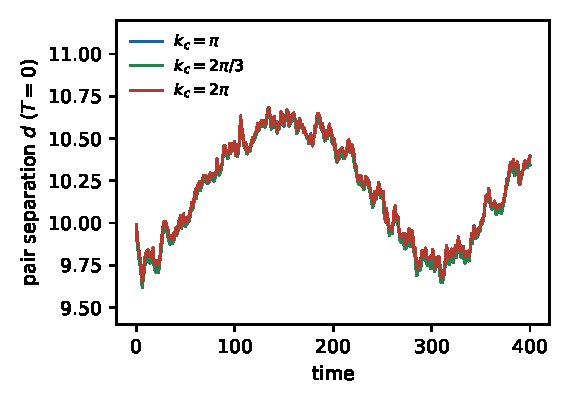
\includegraphics[width=0.52\linewidth]{figures/fl_fig3_T0_known_answer.pdf}
\caption{Known answer: the $T=0$ pair separation at the three cutoffs. Speed $0.1065/0.1068/0.1065$; the curves overlie to $0.5\,\%$.}\label{fig:t0}
\end{figure}

\section{Registered predictions and what happened}\label{sec:results}

\begin{table}[h]\centering\small
\begin{tabular}{lrrrrrr}\toprule
arm ($k_c$, $T$) & runs & $\rho_n/\rho$ & $\alpha$ (energy) & $c=\alpha/(\rho_n/\rho)$ & $\alpha/T$ & $\alpha'$\\\midrule
$2\pi/3$, 0.100 & 6 & 0.0154 & $0.0049\pm0.0008$ & $0.32\pm0.05$ & $0.049\pm0.008$ & $-0.017\pm0.001$\\
$2\pi/3$, 0.216 & 6 & 0.0397 & $0.0121\pm0.0017$ & $0.31\pm0.04$ & $0.056\pm0.008$ & $-0.031\pm0.003$\\
$\pi$, 0.115 & 8 & 0.0270 & $0.0062\pm0.0004$ & $0.229\pm0.015$ & $0.054\pm0.004$ & $-0.010\pm0.002$\\
$\pi$, 0.220 & 6 & 0.0534 & $0.0138\pm0.0023$ & $0.26\pm0.04$ & $0.063\pm0.010$ & $-0.015\pm0.003$\\
$2\pi$, 0.127 & 6 & 0.0709 & $0.0068\pm0.0009$ & $0.096\pm0.013$ & $0.053\pm0.007$ & $-0.005\pm0.002$\\
$2\pi$, 0.173 & 6 & 0.0802 & $0.0096\pm0.0018$ & $0.120\pm0.023$ & $0.055\pm0.011$ & $-0.004$\\\bottomrule
\end{tabular}
\caption{The six arms. Errors are block jackknives over runs; $\alpha'=1-\widehat{(1-\alpha')}$ is the box-frame value, without the $T=0$ pair-size baseline of the preceding paper (all values small and negative; the Iordanskii value would be $+\rho_n/\rho$).}\label{tab:arms}
\end{table}

\begin{failbox}
\textbf{FL2 fails.} The coefficient is $0.31\pm0.03$, $0.232\pm0.014$, $0.102\pm0.011$ at $k_c\xi=2.1$, $3.1$, $6.3$ (weighted over the arms at each cutoff): $(\max-\min)/\mathrm{mean}=0.98$, against the registered $0.2$.
\textbf{The rival fails too:} $c/k_c$ is not constant ($\chi^2=204$ for $2$ degrees of freedom) --- the coefficient \emph{falls} with the cutoff, the Born law makes it rise.
\textbf{FL3's expectation fails} (spread $10$--$30\,\%$). \textbf{One common coefficient fails} ($\chi^2=76$ for $5$ degrees of freedom).
\textbf{FL1 holds} at every cutoff where two temperatures exist ($2\pi/3$: $0.32$, $0.31$; $\pi$: $0.23$, $0.26$; $2\pi$: $0.096\pm0.013$, $0.12\pm0.02$) --- each cutoff is proportional to its own $\rho_n$; it is the coefficient that depends on the cutoff.
\end{failbox}

\begin{figure}[h]\centering
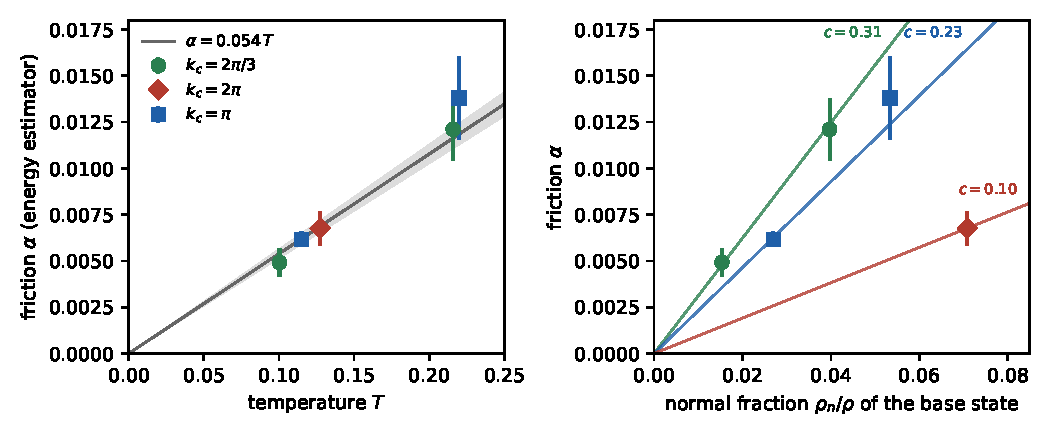
\includegraphics[width=\linewidth]{figures/fl_fig1_alpha_vs_T_and_rho.pdf}
\caption{Left: the friction against temperature, for the three cutoffs; the line is $\alpha=0.054\,T$ (band: one standard error). Right: the same data against the normal fraction of the base state;
the three straight lines through the origin have different slopes (Table~\ref{tab:arms}). Open symbols: fewer than six runs.}\label{fig:alpha}
\end{figure}
\begin{figure}[h]\centering
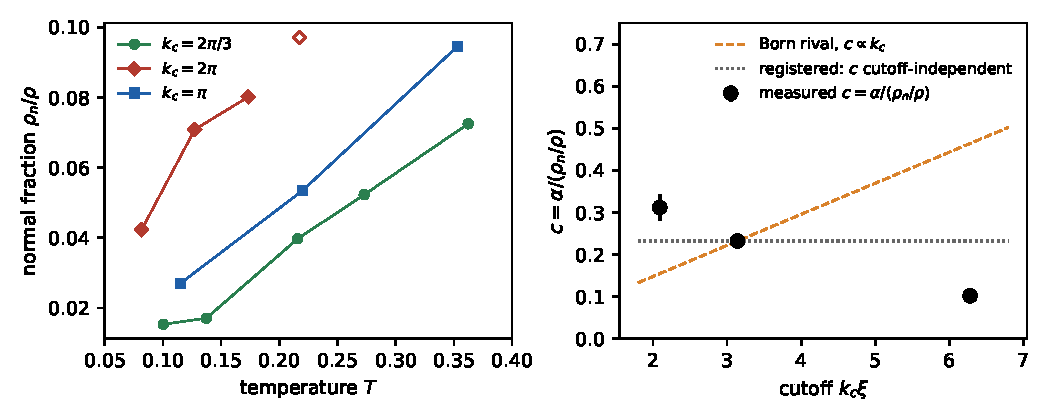
\includegraphics[width=\linewidth]{figures/fl_fig2_lever_and_coefficient.pdf}
\caption{Left: the normal fraction against temperature at the three cutoffs (open: not admitted). Right: the coefficient $c$ against the cutoff: the registered (constant) and rival ($\propto k_c$) predictions fail.}\label{fig:c}
\end{figure}

\section{A temperature law, found after the fact}\label{sec:T}

The comparison of the two panels of Fig.~\ref{fig:alpha} is the finding. At fixed $T$ the friction hardly moves with the cutoff, while $\rho_n/(\rho T)$ moves by a factor of three to four ($0.15$--$0.18$ at $2\pi/3$, $0.24$ at $\pi$, $0.46$--$0.56$ at $2\pi$); $\alpha/T=0.0540\pm0.0026$
in all six arms ($\chi^2=1.28$ for $5$ degrees of freedom, against $76$ for a common $c$). In the earlier paper the three temperatures were at one cutoff, where $\rho_n/\rho\propto T$ (we measured $\rho_n/(\rho T)=0.23$, $0.24$, $0.27$), and
a proportionality to either could not be told from the other; the cutoff scan breaks the degeneracy.

\begin{keybox}
\textbf{Hypothesis H-T} (post hoc; filed as amendment FL-A1 before the last arm was read): $\alpha=a\,T$, $a=0.054\pm0.003$, independent of the cutoff for $k_c\xi\ge2$ (a cutoff at $2.1$ already carries the whole friction).
\textbf{Prediction fixed in advance} for the arm running when it was written ($k_c=2\pi$, $T=0.1734$, $\rho_n/\rho=0.0802$): H-T gives $\alpha_E=0.0094\pm0.0010$; the proportionality to $\rho_n$ at that cutoff's coefficient gives $0.0077$;
$[0.0084,0.0104]$ supports H-T, $[0.0067,0.0087]$ the alternative, the overlap is inconclusive.
\textbf{Outcome} (read 2026-10-09 by the pre-written rule): $\alpha_E=0.0096\pm0.0018$ ($\alpha_{\rm reg}=0.0110\pm0.0014$; six runs, two ended by annihilation, two by track loss), $c=0.120\pm0.023$, $\alpha/T=0.055\pm0.011$ --- \textbf{in the window of H-T}, outside that of the $\rho_n$ law (inclusion by the rule; by itself the arm lies $0.2\sigma$ from $0.0094$ and $1.0\sigma$ from $0.0077$).
\end{keybox}

\paragraph{Estimator robustness (found while porting the estimators to Rust).} A re-implementation of the registered estimators in a second language, bit-identical to the Python on four real tracks, was run on the registered synthetic gate over many seeds
and showed that the energy estimator of $\alpha$, the primary estimator used throughout, is \emph{biased low by the diffusion}: for a true $\alpha=0.02$ it returns $0.0200$ without diffusion and $0.0183$, $0.0163$, $0.0156$ at $\eta=5\times10^{-4}$, $10^{-3}$, $2\times10^{-3}$
($-8$, $-18$, $-22\,\%$), independently of the detection noise, while the regression estimator is unbiased ($0.0194$); the registered gate passed on one seed. In the data the two estimators differ by $5$--$21\,\%$ in that direction. With the regression estimator
$\alpha/T=0.0598\pm0.0023$ ($\chi^2=5.2$ for $5$ degrees of freedom; $0.0540\pm0.0026$ with the energy estimator) and the coefficient $c$ is $0.355\pm0.035$, $0.250\pm0.012$, $0.124\pm0.011$ at the three cutoffs, a factor $2.9$: every conclusion above stands, with
absolute values of $\alpha$ higher by about $11\,\%$ (the values quoted for $k_c=\pi$ in the preceding paper are low by $5$--$20\,\%$).

\paragraph{Why a temperature law is natural, and what it requires.} In a classical field every mode carries the energy $T$, so occupations are $n_k=T/\varepsilon_k$ and anything linear in the occupation is linear in $T$. The kinetic form
$D=\tfrac12\!\int\!\frac{d^2k}{(2\pi)^2}\,\frac{T}{\varepsilon_k^2}\,k^2c_g\sigma_{\rm tr}$ with the Bogoliubov energy $\varepsilon_k=\sqrt{k^2+k^4/4}$ is then $T$ times a function of the cutoff;
for $k\xi\gg1$ ($\varepsilon\simeq k^2/2$, $c_g\simeq k$) the integrand is $\propto\sigma_{\rm tr}(k)$, so a drag that does not depend on the cutoff beyond $k_c\xi\simeq2$ requires $\int^\infty\sigma_{\rm tr}\,dk$ to converge --- a transport cross-section
falling faster than $1/k$ --- whereas the same weights make $\rho_n$ grow logarithmically with the cutoff. This is a constraint on the scatterer if the independent-mode picture holds; the long-wavelength Born cross-section $\sigma_\parallel=\kappa^2k/8c^2$ grows
linearly with $k$ and is valid for fewer than $3\,\%$ of the modes of a cutoff $\pi$~\cite{Sonin1997}, so it cannot be extrapolated. The direct measurement of $\sigma_{\rm tr}(k)$ --- a monochromatic Bogoliubov wave scattered by one vortex at $T=0$ --- would settle it and is the obvious next experiment.

\section{What this corrects}\label{sec:corrects}

\begin{enumerate}[nosep]
\item The statement ``$\alpha\simeq0.24\,\rho_n/\rho$'' of the preceding paper~\cite{Callens2026a} holds at $k_c=\pi$ only; the relation that survives the cutoff scan is $\alpha=0.054\,T$ (confirmed on the last arm by the registered rule).
\item The reading of $0.24$ as a mode-averaged transport cross-section of the vortex, $\langle c_g\sigma_{\rm tr}\rangle=1.4\,\xi$, ``the geometric size of the core'', is withdrawn: the same quantity is $1.9$, $1.4$, $0.59\,\xi$ at the three cutoffs. The identity of Appendix~\ref{app:lean} stands; its coefficient is a property of the bath's mode set, not of the vortex.
\item The recommendation to compare with quantum gases at equal $\rho_n/\rho$ rather than equal $T/T_c$ is withdrawn in the same sense: in this model $\rho_n/\rho$ depends on the cutoff, $\alpha$ does not. (A comparison with experiment needs a map from the classical-field temperature to the physical one, and that map itself depends on the cutoff; the claim here is internal to the model.)
\end{enumerate}

\section{Limits}\label{sec:limits}

One box ($L=64$), one interaction strength ($mg=1$), pairs of two sizes and two or three temperatures per cutoff; the two new cutoffs at one and two temperatures; the dependence on the pair size ($\alpha$ larger for $d_0=12$ than for $d_0=8$ by $38$--$85\,\%$ at the new cutoffs, not at $\pi$) and the small negative transverse coefficient, whose magnitude grows toward the coarse cutoff ($\alpha'=-0.005$ at $2\pi$, $-0.010$ and $-0.015$ at $\pi$, $-0.017$ and $-0.031$ at $2\pi/3$; always far from the Iordanskii value) are reported and unexplained --- either a bias of the energy estimator at the coarse cutoff or a finite-pair effect. The cutoff $2\pi/3$ shares its grid with $\pi$ and the cutoff $2\pi$ has a finer grid: a lattice-spacing effect is not excluded by this design, though the $T=0$ pair is insensitive to it to $0.3\,\%$.
The energy estimator of $\alpha$ is biased low by diffusion (above), so the absolute coefficient is $0.054$--$0.060$; the law is estimator-independent in its form. The temperature law was formulated after five arms were read and confirmed by the rule on the sixth, whose error is large; it is a well-supported empirical relation over $T=0.10$--$0.22$ and three cutoffs, not a derived one, and it has not been tested above $T=0.22$ (where thermal vortices enter) or at other box sizes or interaction strengths.

\section{Conclusion}

A pre-registered test failed in the way that matters: the coefficient between the friction and the normal density is not a property of the vortex, and neither the registered cutoff-independence nor its Born rival describes it. What the
test found instead is a friction that follows the temperature and ignores the cutoff over a factor three, which
is a stricter statement than the one it replaces, and a correction of the preceding paper's reading, made here rather than left to a reader.

\paragraph{Data and code availability.} Pre-registrations, results logs, the ledger (claims 089--098), analysis scripts, the Lean sources and the figure scripts are in the repository \url{https://github.com/xaviercallens/SocrateAI-Scientific-QuantumFluids} (scripts as of commit \texttt{2ff887a4f57a}); the numerical record up to the preceding paper is archived in~\cite{Callens2026sw}. The pure-Rust re-implementation of the engine and estimators that exposed the estimator bias is in the rusty-SUNDIALS crate \texttt{qf-pgpe}.

\appendix
\section{Registered items and outcomes}\label{app:protocol}
\begin{center}\small\begin{tabular}{p{0.18\linewidth}p{0.42\linewidth}p{0.3\linewidth}}\toprule
item & registered (before any run) & outcome\\\midrule
FL1 & $\alpha\propto\rho_n$ at each cutoff & holds at all three cutoffs (each to its own $\rho_n$)\\
FL2 & $c$ within $20\,\%$ across cutoffs & fails (spread $0.98$)\\
Born rival & $c\propto k_c$ & rejected ($\chi^2=204/2$)\\
FL3 & spread $10$--$30\,\%$, $c(2\pi/3)\le c(\pi)\le c(2\pi)$ & fails (ordering reversed)\\
$T=0$ control & speed within $4\,\%$, $|\alpha|\le10^{-3}$ & passes at all cutoffs; $\eta$ floor marginal at $2\pi/3$\\
G0 energy criterion & $\alpha_E$ within $15\,\%$ (one numpy seed) & passes on 2 of 12 seeds: biased low by diffusion (regression unbiased)\\
base admission & raw $n_v<0.5$ & fine $T=0.217$ base fails; replaced by $T=0.173$ (admitted, $n_v=0.08$)\\
H-T & post hoc, FL-A1 & consistent ($\chi^2=1.28/5$); registered window for the last arm met ($0.0096$ in $[0.0084,0.0104]$)\\\bottomrule\end{tabular}\end{center}

\section{Lean}\label{app:lean}
\lean{FrictionKinetic}: for a finite set of modes with nonnegative weights $w_k$ and drag factors $f_k=c_g\sigma_{\rm tr}$, $D=\sum w_kf_k$ and $\rho_n=\sum w_k$ give
$\alpha/(\rho_n/\rho)=\tfrac{\rho}{\rho_s\kappa}\cdot\sum w_kf_k/\sum w_k$ (an identity), the weighted mean lies between $\min f$ and $\max f$, and for equal weights (Rayleigh--Jeans with a phonon dispersion) it is
the arithmetic mean. Nothing about the value of $\sigma_{\rm tr}$ or its dependence on $k$ is asserted; that is the measurement.

\section{Code}\label{app:code}
The analysis (\texttt{exploration/pgpe/analyze\_friction\_law.py}) applies the registered estimators to every arm and writes the verdict file; the core of the cutoff comparison is
\begin{lstlisting}
def wmean(v, s):
    v, s = np.array(v), np.array(s); w = 1 / s ** 2; m = (w * v).sum() / w.sum()
    return float(m), float(1 / np.sqrt(w.sum())), float(((v - m) ** 2 * w).sum())   # mean, se, chi2

c_by_cutoff = {k: wmean([x["c_energy"] for x in v], [x["c_energy_se"] for x in v]) for k, v in arms_by_cutoff.items()}
spread = (max(m for m, _, _ in c_by_cutoff.values()) - min(m for m, _, _ in c_by_cutoff.values())) / mean_of_means   # FL2: < 0.20
m_T, se_T, chi2_T = wmean([a["alpha_energy_over_T"] for a in arms], [a["alpha_energy_over_T_se"] for a in arms])   # H-T
\end{lstlisting}
Data, scripts, pre-registrations and the ledger: \cite{Callens2026sw}.

\bibliographystyle{unsrt}
\bibliography{refs_vortex_transport}
\end{document}
